\documentclass[paper=128mm:96mm, fontsize=11pt, pagesize, parskip=half-,]{scrartcl}

\linespread{1.12} % Increase line spacing for readability

% Colors
\usepackage{xcolor}
\definecolor{generalcolor}{RGB}{52,73,94}
\definecolor{myblue}{HTML}{268BD2}
\definecolor{mygreen}{HTML}{859900}
\definecolor{mygray}{HTML}{93A1A1}

% Margins
\usepackage[includeheadfoot, top=3.5mm, bottom=3.5mm, left=5.5mm, right=5.5mm, headsep=6.5mm, footskip=8.5mm]{geometry}

% Fonts
\usepackage[T1]{fontenc}
\usepackage{lmodern}
\renewcommand{\familydefault}{\sfdefault}

% Various required packages
\usepackage{amsthm} % Required for theorem environments
\usepackage{bm} % Required for bold math symbols (used in the footer of the slides)
\usepackage{graphicx} % Required for including images in figures
\usepackage{tikz} % Required for colored boxes
\usepackage{booktabs} % Required for horizontal rules in tables
\usepackage{multicol} % Required for creating multiple columns in slides
\usepackage{lastpage} % For printing the total number of pages at the bottom of each slide
\usepackage[english]{babel} % Document language - required for customizing section titles
\usepackage{microtype} % Better typography
\usepackage{tocstyle} % Required for customizing the table of contents
\usepackage[toc]{multitoc}
\usepackage{fontspec}
\usepackage{listings}
\usepackage{calc}

\lstset{ %
  basicstyle=\footnotesize,        % the size of the fonts that are used for the code
  breaklines=true,                 % sets automatic line breaking
  captionpos=b,                    % sets the caption-position to bottom
  commentstyle=\color{mygreen},    % comment style
  escapeinside={\%*}{*)},          % if you want to add LaTeX within your code
  frame=none,                      % adds a frame around the code
  keywordstyle=\color{blue},       % keyword style
  language=Python,                 % the language of the code
  numbers=left,                    % where to put the line-numbers; possible values are (none, left, right)
  numbersep=5pt,                   % how far the line-numbers are from the code
  numberstyle=\tiny\color{mygray}, % the style that is used for the line-numbers
  rulecolor=\color{black},         % if not set, the frame-color may be changed on line-breaks within not-black text (e.g. comments (green here))
  stepnumber=2,                    % the step between two line-numbers. If it's 1, each line will be numbered
  showspaces=false,
  tabsize=2,                       % sets default tabsize to 2 spaces
  title=\lstname,                   % show the filename of files included with \lstinputlisting; also try caption instead of title
  xleftmargin=.02\textwidth
}


\theoremstyle{definition}
\newtheorem{definition}{Definition}[section]

\newcommand*{\lowbiglquote}[1][70]{%
  \setbox0=\hbox{\fontsize{#1}{0}\selectfont``}%
  \setlength{\dimen0}{\ht0 - \heightof{A}}%
  \noindent\llap{\smash{\lower\dimen0\box0 }}}

\newcommand*{\lowbigrquote}[1][70]{%
  \setbox0=\hbox{\fontsize{#1}{0}\selectfont''}%
  \setlength{\dimen0}{\ht0 - \heightof{A}}%
  \unskip\rlap{\smash{\lower\dimen0\box0 }}}

\newenvironment{Figure}
  {\par\medskip\noindent\minipage{\linewidth}}
  {\endminipage\par\medskip}

\newcommand*{\centerinpage}[1]{
	\null \vfill
	\begin{Figure}
		\centering	
		#1	
	\end{Figure}
	\vfill \null}

% Slide layout configuration
\usepackage{scrpage2} % Required for customization of the header and footer
\pagestyle{scrheadings} % Activates the pagestyle from scrpage2 for custom headers and footers
\clearscrheadfoot % Remove the default header and footer
\setkomafont{pageheadfoot}{\normalfont\color{black}\sffamily} % Font settings for the header and footer

% Sets vertical centering of slide contents with increased space between paragraphs/lists
\makeatletter
\renewcommand*{\@textbottom}{\vskip \z@ \@plus 1fil}
\newcommand*{\@texttop}{\vskip \z@ \@plus .5fil}
\addtolength{\parskip}{\z@\@plus .25fil}
\makeatother

% Remove page numbers and the dots leading to them from the outline slide
\makeatletter
\newtocstyle[noonewithdot]{nodotnopagenumber}{\settocfeature{pagenumberbox}{\@gobble}}
\makeatother
\usetocstyle{nodotnopagenumber}
\setcounter{tocdepth}{1}

\AtBeginDocument{\renewcaptionname{english}{\contentsname}{\Large Outline}}

% Header configuration - if you don't want a header remove this block
\ihead{
\hspace{-2mm}
\begin{tikzpicture}[remember picture,overlay]
\node [xshift=\paperwidth/2,yshift=-\headheight] (mybar) at (current page.north west)[rectangle,fill,inner sep=0pt,minimum width=\paperwidth,minimum height=2\headheight,top color=generalcolor,bottom color=generalcolor]{};
\end{tikzpicture}
\color{white}\runninghead
} % Header text defined by the \runninghead command below and colored white for contrast

% Footer configuration
\setlength{\footheight}{8mm} % Height of the footer
\addtokomafont{pagefoot}{\footnotesize} % Small font size for the footnote

\ifoot{% Left side
\hspace{-2mm}
\begin{tikzpicture}[remember picture,overlay]
\node [xshift=\paperwidth/2,yshift=\footheight] at (current page.south west)[rectangle,fill,inner sep=0pt,minimum width=\paperwidth,minimum height=2pt,top color=generalcolor,bottom color=generalcolor]{}; % Green bar
\end{tikzpicture}
\myauthor\ \raisebox{0.2mm}{$\bm{\vert}$}\ \myuni % Left side text
}

\ofoot[\pagemark/\pageref{LastPage}\hspace{-2mm}]{\pagemark/\pageref{LastPage}\hspace{-2mm}} % Right side

% Section spacing - deeper section titles are given less space due to lesser importance
\usepackage{titlesec} % Required for customizing section spacing
\titlespacing{\section}{0mm}{0mm}{0mm} % Lengths are: left, before, after
\titlespacing{\subsection}{0mm}{0mm}{-1mm} % Lengths are: left, before, after
\titlespacing{\subsubsection}{0mm}{0mm}{-2mm} % Lengths are: left, before, after
\setcounter{secnumdepth}{0} % How deep sections are numbered, set to no numbering by default - change to 1 for numbering sections, 2 for numbering sections and subsections, etc

% The code for the box which can be used to highlight an element of a slide (such as a theorem)
\newcommand*{\mybox}[2]{ % The box takes two arguments: width and content
\par\noindent
\begin{tikzpicture}[mynodestyle/.style={rectangle,draw=generalcolor,thick,inner sep=2mm,text justified,top color=white,bottom color=white,above}]\node[mynodestyle,at={(0.5*#1+2mm+0.4pt,0)}]{ % Box formatting
\begin{minipage}[t]{#1}
#2
\end{minipage}
};
\end{tikzpicture}
\par\vspace{-1.3em}}

\newcommand*{\myfullpage}[2] {
\thispagestyle{empty}
\begin{tikzpicture}[remember picture,overlay] % Background box
\node [xshift=\paperwidth/2,yshift=\paperheight/2] at (current page.south west)[rectangle,fill,inner sep=0pt,minimum width=\paperwidth,minimum height=\paperheight/3,top color=generalcolor,bottom color=generalcolor]{}; % Change the height of the box, its colors and position on the page here
\end{tikzpicture}
% Text within the box
\begin{flushright}
\vspace{15mm}
\color{white}\sffamily
{\bfseries\Large #1\par}
\vspace{0.2cm}
\large
#2
\vfill
\end{flushright}}

% PRESENTATION INFORMATION
\newcommand*{\mytitle}{Introduction to SOFA + BDAE}
\newcommand*{\runninghead}{SOFA + BDAE}
\newcommand*{\myauthor}{Steffen Karlsson}
\newcommand*{\mydate}{\today}
\newcommand*{\myuni}{University of Copenhagen -- eScience, NBI}

\newcommand*{\newslide}{\clearpage}

\begin{document}

% Title slide - you may have to tweak a few of the numbers if you wish to make changes to the layout
\thispagestyle{empty} % No slide header and footer
\begin{tikzpicture}[remember picture,overlay] % Background box
\node [xshift=\paperwidth/2,yshift=\paperheight/2] at (current page.south west)[rectangle,fill,inner sep=0pt,minimum width=\paperwidth,minimum height=\paperheight/3,top color=generalcolor,bottom color=generalcolor]{}; % Change the height of the box, its colors and position on the page here
\end{tikzpicture}
% Text within the box
\begin{flushright}
\vspace{0.6cm}
\color{white}\sffamily
{\bfseries\Large\mytitle\par} % Title
\vspace{0.5cm}
\normalsize
\myauthor\par % Author name
\mydate\par % Date
\vfill
\end{flushright}

\newslide

% TABLE OF CONTENTS
\thispagestyle{empty}
\small\tableofcontents
\newslide

% PRESENTATION SLIDES
\centerinpage{
	{\color[rgb]{0.74,0.76,0.78} This page has intentionally been left blank}
}
\newslide

\subsection{Data residual}
\centerinpage{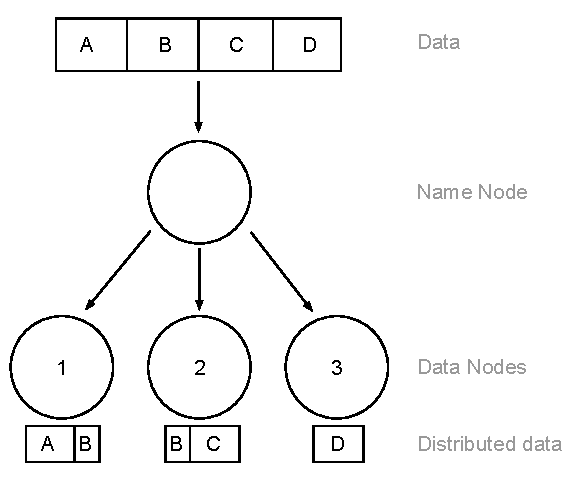
\includegraphics[scale=0.6]{../Report/pdf/data-residual.pdf}}
\newslide

\section{Problem definition}
\centerinpage{
\begin{center}
\mybox{0.8\textwidth}{
	\textit{First and foremost, analyze and investigate whether a distributed parallel file system that efficiently hides latency and reduce IO-cost is durable. Secondly, if achievable implement a prototype in a sensibly selected language, architecture and environment.}}
\end{center}}
\newslide

\section{Proposal}
\textbf{Goal:} Design and implement a prototype of an alternative to the existing file archives used in big data analysis subsequently.

\textbf{Outcome: } A substitute system eliminating data residuals and with reduced I/O-cost, complexity and increased performance.

\textbf{By: } Splitting data semantically consistent at key positions, thus data will be divided into arbitrarily sized chunks instead of fixed.

\textbf{Challenges: } Describing a domain specific model to characterize the data semantics and defining a direct data mapping for storing and retrieval.
\newslide

%\begin{multicols}{2}
\subsection{Assumptions}
\begin{itemize}
	\item Solution is targeted research + scientific related data and used for BDA
	\item Data entries can be processed and analyzed independently
	\item Whole datasets is accessed, processed or modified at once
	\item Majority of the datasets is passive
\end{itemize}

%\columnbreak

%\subsection{Expected results}
%\begin{itemize}
%	\item 
%\end{itemize}
%\end{multicols}

\newslide

\section{Analysis}

BDA is widely used in most research areas and the volume, variety, and velocity that data are progressing will continue expanding. The demand for processing huge amount data has never been larger.

\begin{multicols}{2}
\begin{quotation}
\vspace*{1mm}
\lowbiglquote[30] \textit{$\ldots$ rather heavyweight and difficult to adapt to custom environments } \lowbigrquote[30]
\end{quotation}
\qquad\qquad \tiny{[P. Mundkur, V. Tuulos, and J. Flatow]}

\columnbreak

\normalsize{\textbf{Glenn Lockwood: } Hadoop isn’t designed with HPC in mind and is developed under other circumstances, and for another purpose than what it is used for nowadays.}
\end{multicols}
\newslide

\subsection{Single Master}
\begin{multicols}{2}
\centerinpage{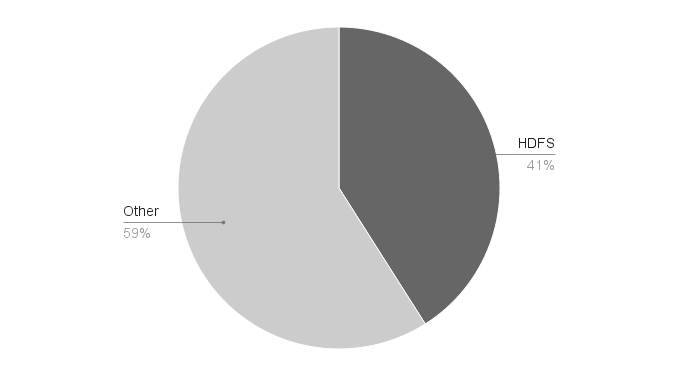
\includegraphics[scale=0.28]{../Report/img/fb-hadoop-incidents.png}}
\columnbreak

\begin{quotation}
\vspace*{1mm}
\lowbiglquote[25] \footnotesize{\textit{ $\ldots$ if that machine or process became unavailable, the cluster as a whole would be unavailable until the NameNode was either restarted or brought up on a separate machine. }} \lowbigrquote[25]
\end{quotation}

\begin{quotation}
\vspace*{1mm}
\lowbiglquote[25] \footnotesize{\textit{The permanent loss of NameNode data would render the cluster's HDFS inoperable. }} \lowbigrquote[25]
\end{quotation}

\end{multicols}

\newslide
\textbf{Facebook avatar node (solution)}

\begin{Figure}
\centering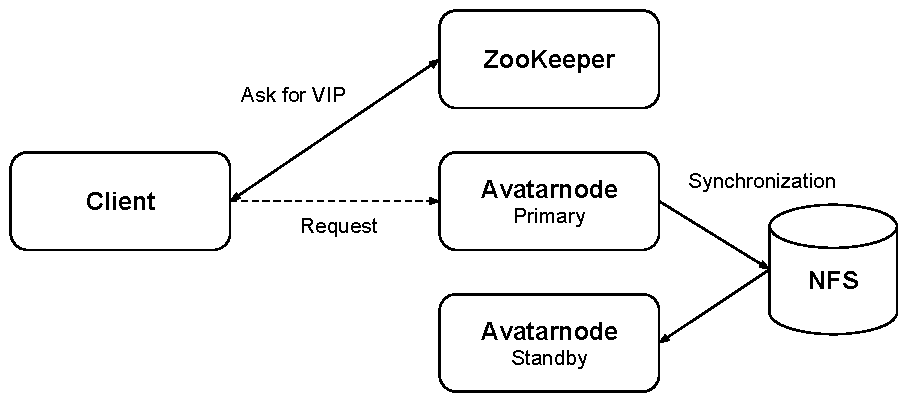
\includegraphics[scale=0.42]{../Report/pdf/facebook-avatarnode.pdf}
\end{Figure}
\begin{itemize}
	\item 50\% lesser planned downtime, \textit{i.e.}, a critical time where that part of the warehouse is unavailable
\end{itemize}

\textbf{Problems: } Single point of failure error reliability of the Apache ZooKeeper instance and of the NFS.
\newslide

\textbf{Hadoop 2.x (solution)}
\begin{multicols}{2}
Full redundant duplication of the NameNode (active and standby), thus Fast fail-over.
\vspace*{2mm}

\textbf{Synchronization achieved by:}
\begin{enumerate}
	\item Quorum Journal Manager
	
	Minimum 3 daemons: each modification has to be written to a quorum based majority of the synchronization daemons.
	\vfill \null
	\columnbreak
	
	\item NFS storage synchronization (similar to Facebooks solution)
	\centerinpage{
		\begin{Figure}
			\centering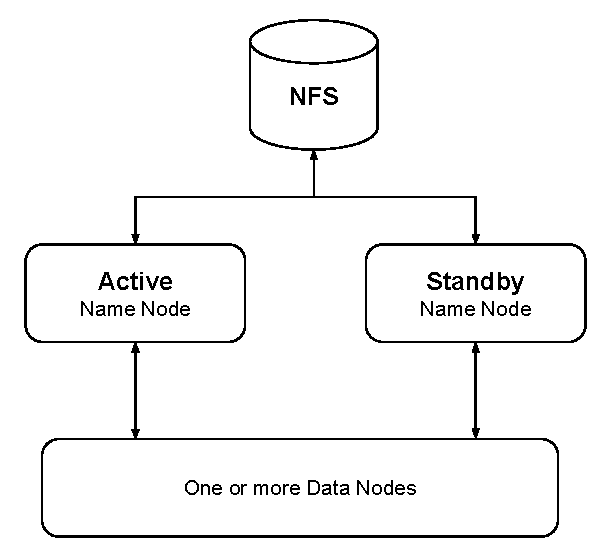
\includegraphics[scale=0.42]{../Report/pdf/hadoop-2x-nfs.pdf}
		\end{Figure}
	}
\end{enumerate}

\end{multicols}

\newslide

\begin{multicols}{2}

\subsection{Presumptions}
\begin{itemize}
	\item Operating in a homogeneous and high-performance computing environment like a cluster
	\item Minimal replication scheme
	\item Reduced security priority within the system
\end{itemize}
\vfill \null

\columnbreak
\subsection{Objectives}
\begin{itemize}
	\item Semantically coherent parts are stored jointly, thus eliminating the data residual problem
	\item Arbitrary sized chunks
	\item Eliminating single-point of failure
	\item Transparent but suitable load balancing protocol
\end{itemize}
\vfill \null

\end{multicols}
\newslide

\subsection{Examples}
Three different types of datasets, which combined will contribute to an \newline exploratory research and will challenge various critical aspects.

\textbf{Image data: }
\vspace*{-2mm}
\begin{itemize}
	\item Limited to high-resolution grayscale X-rays.
	\item Datasets with fixed sized chunks and thus enabling the opportunity of precisely calculating positions and offsets
\end{itemize}

\textbf{Text: }
\vspace*{-2mm}
\begin{itemize}
	\item Books and readily available raw news articles
	\item Semantic data correlation
	\item Support for arbitrary sized blocks
\end{itemize}

\textbf{Simulation results: }
\vspace*{-2mm}
\begin{itemize}
	\item Astrophysics and climate modeling data
	\item Large complex and multidimensional scientific data
	\item Data transformation
	\item Feature extraction
\end{itemize}
\newslide

\section{Architecture and design}
Modeling an interpretation of a Storage Area Network (SAN)
\begin{Figure}
	\centering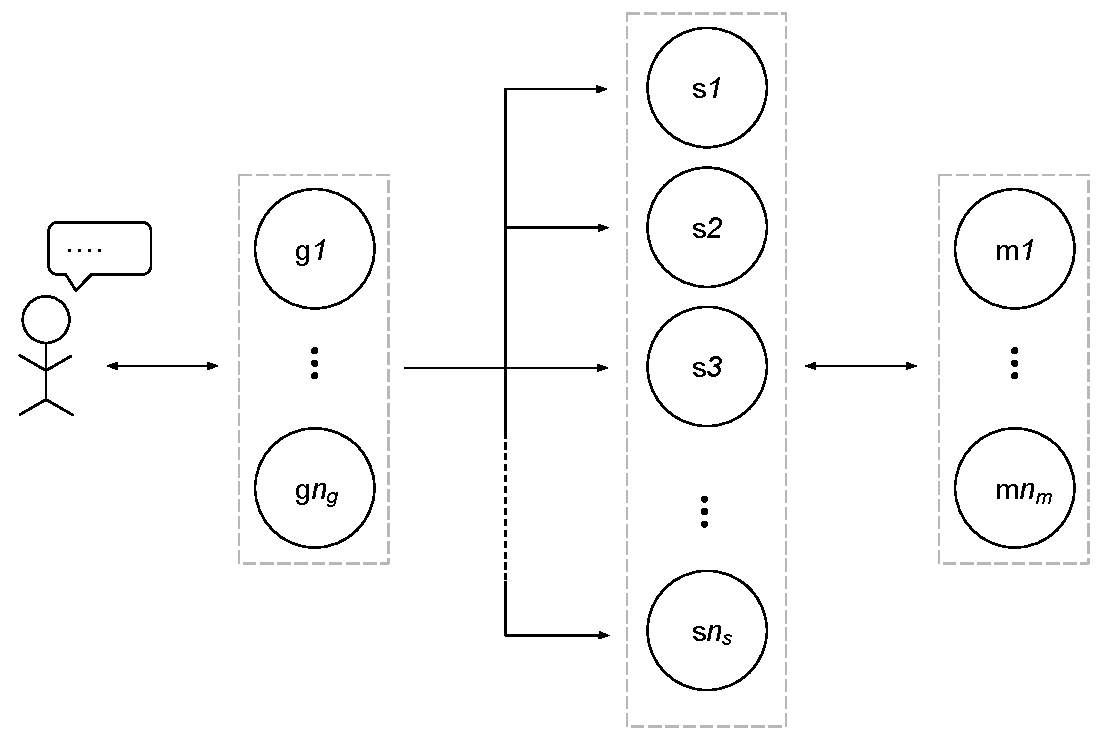
\includegraphics[scale=0.38]{../Report/pdf/sofa-overview.pdf}
\end{Figure}
\newslide

\subsection{Architectural style}
Modeling the notion of a hybrid related distributed with:
\begin{itemize}
	\item Decentralized collection of interconnected storage nodes, reflecting a \newline zero-hop distributed hash table ring, thus providing full data consistency.
	\item Potentially multiple stateless gateway servers
	\item One or more observation monitors
\end{itemize}

\centerinpage{
	\begin{Figure}
		\centering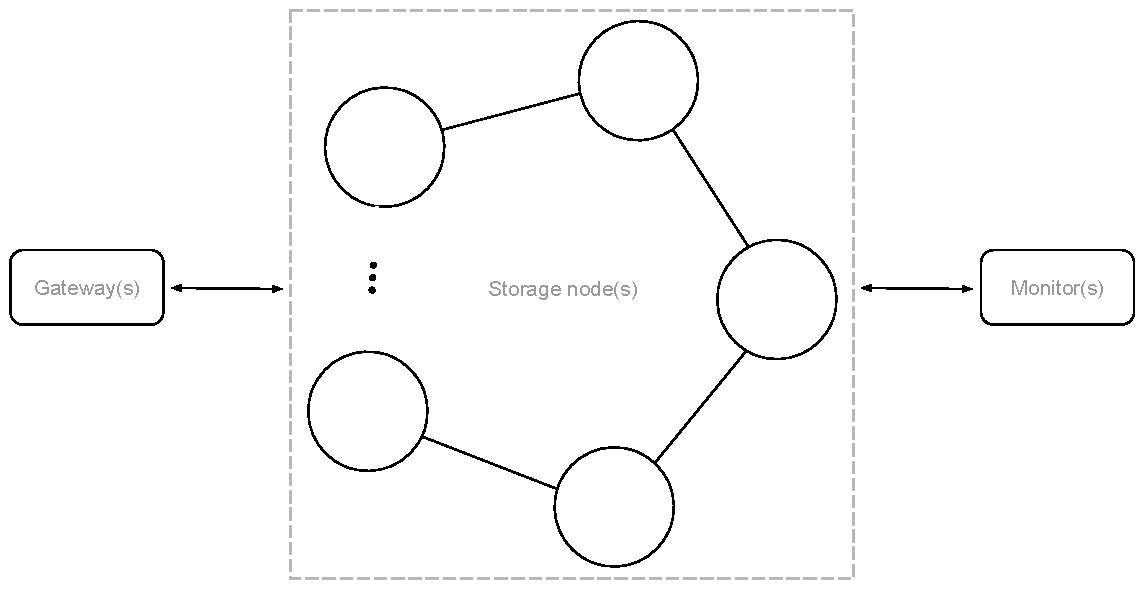
\includegraphics[scale=0.5]{../Report/pdf/architecture-overview.pdf}
	\end{Figure}
}

\newslide

\subsection{Partitioning and distribution}
Implementing a simple, fair share and starvation free load balancing algorithm
\begin{Figure}
	\centering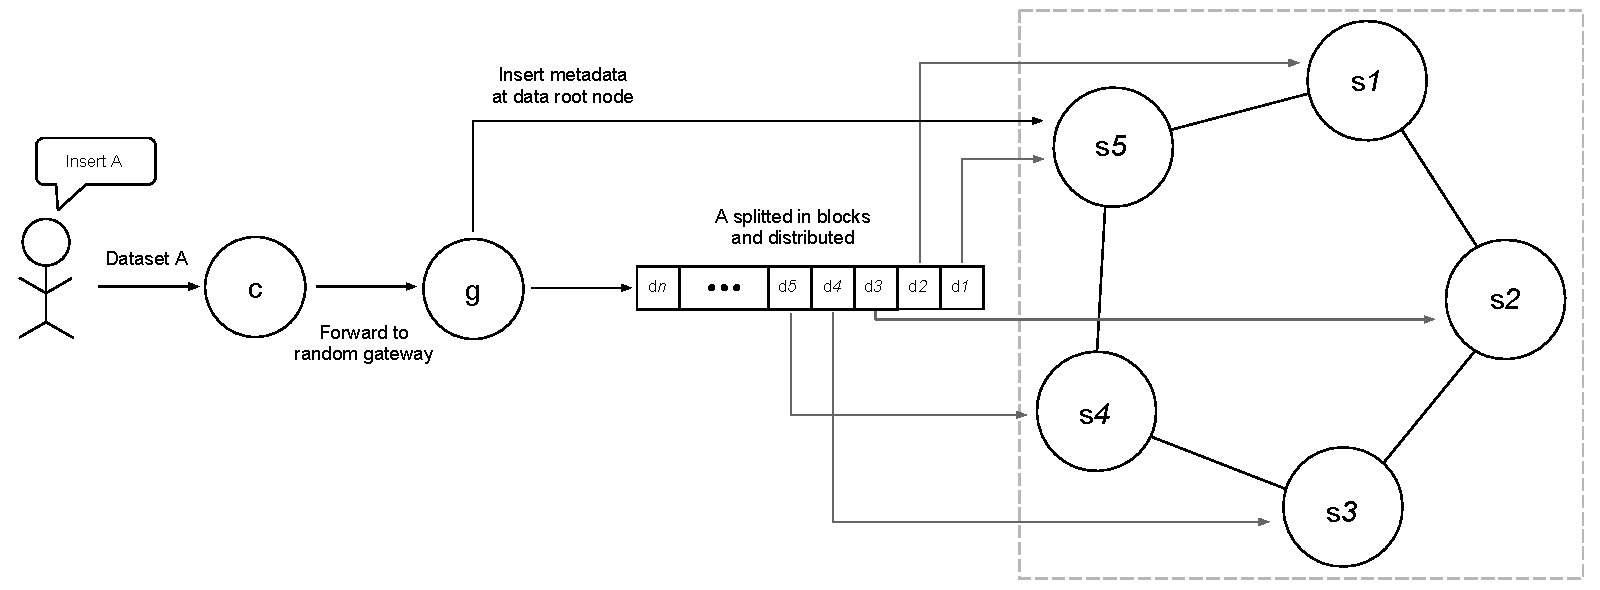
\includegraphics[scale=0.32]{../Report/pdf/rr-partitioning.pdf}
\end{Figure}	
\textbf{Downside:} State, availability and workload etc. isn't considered.

\textbf{Alternatives:} Other alternatives such as \textit{"Linear"} and \textit{"Chucked"} is supported.
\newslide

\subsection{Naming and virtualization}
\begin{itemize}
	\item Unique global name for each instance
	\item Different elements/components identified using a predominantly structured naming based technique:
		
	\quad \textbf{Nodes:} \texttt{sofa}:<instance name>:<type ref>:<sequence number>

	\quad \textbf{Data:} <instance name>:<data type>:<sequence number>
	
	\item Each semicolon denotes an explicit and more specific context
	\item Hashing is used to generate anonymous unique identifier $\rightarrow$ entries in the user-specific limited zero-hop distributed hash table.
\end{itemize}
\newslide

\subsection{Security}
\begin{itemize}
	\item Trusted environment, like Amazon Dynamo.
	\item Data integrity and security have predominantly been given low priority.
	\item Security evidently an influential component from the outside, when handling user inputs.
\end{itemize}
\newslide

\section{General implementation details}
\begin{itemize}
	\item Implemented in Python
	\item Communication at the moment implemented as Pyro4 RPC.
	\item Disks are emulated as shelves.
	\item Installable by setup tools + PIP and provided \texttt{install.sh} script.
	\item Bootable components by \texttt{boot.sh}:
	
	\quad \texttt{sh boot.sh sofa.cfg gateway storage}
\end{itemize}
\newslide

\section{System configuration}
\vspace*{3mm}
\begin{lstlisting}[language=bash, frame=single, basicstyle=\ttfamily\tiny, otherkeywords={[,],=}]
[general]
project-path = /code/sofa-project/sofa
log-file = /code/sofa-project/sofa.log
keyspace-size = 2**5
instance-name = textdata
heartbeat-scheduler-delay = 1  # Defined in seconds
block-size = 2.906020  # Defined in megabytes

[gateway]
addresses = localhost:9999

[storage]
addresses = localhost:8888, localhost:8887, localhost:8886

[monitor]
addresses = localhost:7777
\end{lstlisting}
\newslide

\section{Core API}
\begin{itemize}
	\item Create/update dataset
	\begin{lstlisting}[language=Python, basicstyle=\ttfamily\tiny, numbers=none]
	def create(self, name, package, extra_meta_data=None)
	\end{lstlisting}
	\vspace*{-5mm}
	\item Append
	\begin{lstlisting}[language=Python, basicstyle=\ttfamily\tiny, numbers=none]
	def append(self, name, path_or_url)
	\end{lstlisting}
	\vspace*{-5mm}	
	\item Submit / Poll for result
	\begin{lstlisting}[language=Python, basicstyle=\ttfamily\tiny, numbers=none]
	def submit_job(self, name, function, query)
	
	def poll_for_result(self, name, function, query)
	\end{lstlisting}
\end{itemize}
\newslide

\section{\texttt{SofaBaseObject}}
A set of abstract methods to be overridden in order to define a dataset context.

\begin{lstlisting}[language=Python, basicstyle=\ttfamily\tiny, numbers=none]
def preprocess(self, data_ref)

# default: Does nothing
def postprocess(self, res)

def get_operations(self)

def next_entry(self, data)

# default: Round robin
# options: Chuncked and Linear
def get_distribution_strategy(self)

# default and required: Check if its a keyword function
def verify_function(self, function_name)
\end{lstlisting}
\newslide

\section{Operation}
Context for describing a job to submit to SOFA.
\vspace*{-1mm}
\begin{itemize}
	\item (A)symmetric left/right semantic unit ghosts
	\item Multiple arguments
	\item Full or customizable shorthand syntax
\end{itemize}
\vspace*{5mm}
\begin{center}
\begin{lstlisting}[language=Python, basicstyle=\ttfamily\tiny, numbers=none, showtabs=false, showstringspaces=false, showspaces=false, otherkeywords={[,{,},],Sequential,Parallel}]
    '[{[occurrences, sum], [occurrences_no_case, sum]}, equality]'


     Sequential(Parallel(Sequential(count_occurrences, sum),
                         Sequential(count_occurrences_no_case, sum)), equality)
\end{lstlisting}
\end{center}
\newslide

\myfullpage{SOFA Applications}{Big Data Analysis Engine}
\newslide

\section{BDAE}
User tier based semantic aware MapReduce framework application, built on top on the available SOFA textbf{Core API}

\subsection{User tiers}
\begin{itemize}
	\item \textbf{Data scientist}: Submit new job and poll for result
	\item \textbf{Data manager}: Create and modify datasets
	\item \textbf{SysAdmin}: (Re)boot and take down servers and services.
\end{itemize}

\newslide

\subsection{MapReduce dataset}
Abstract but more specific implementation of the general \texttt{SofaBaseObject}, targeting MapReduce operations.
\vspace*{2mm}
\begin{lstlisting}[language=Python, basicstyle=\ttfamily\tiny, numbers=none]
def get_map_functions(self)
def get_reduce_functions(self)

# Implemented as: Check if its a keyword function and check that the the functions
# specified are part of the map and reduce functions listed.
def verify_function(self, function_name)
\end{lstlisting}
\vspace*{-3mm}
\footnotesize{Functions not described above from \texttt{SofaBaseObject} are still abstract and has to be implemented in an application specific context.}

\subsection{Collection}
Group of individual datasets within the same research or scientific context.
\newslide

\subsection{MapReduce Implementation}
\vspace*{-6mm}
\centerinpage{\includegraphics[scale=0.33]{../Report/pdf/submit_job.pdf}}

\centerinpage{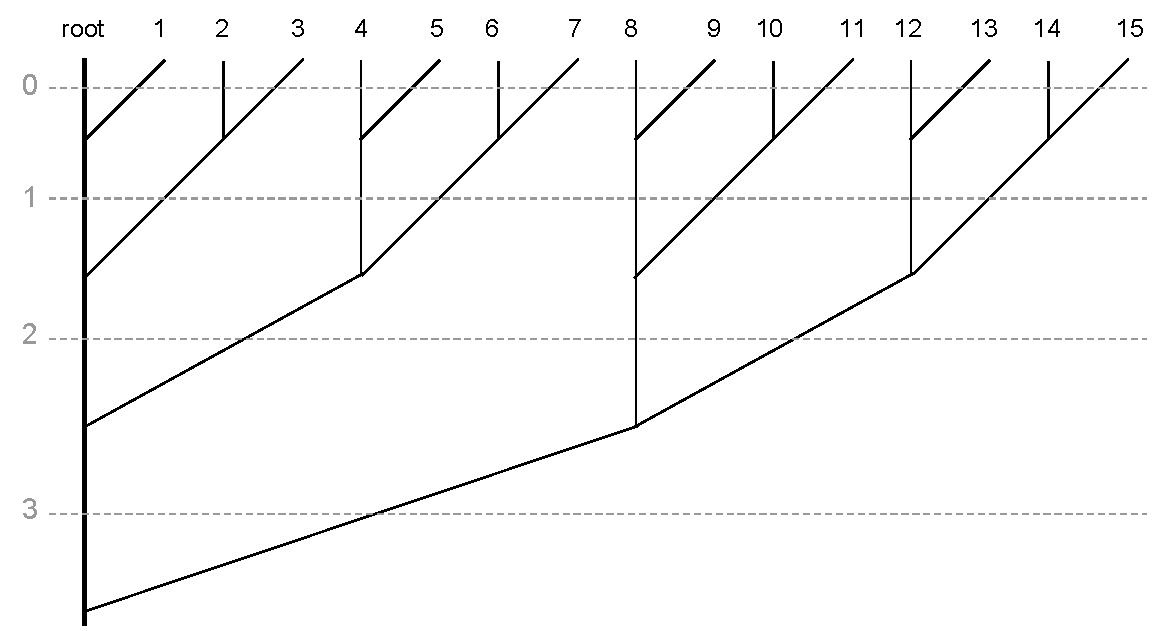
\includegraphics[scale=0.45]{../Report/pdf/reduction_tree.pdf}}
\newslide

\subsection{Templates}
\begin{itemize}
	\item Text dataset with word or sentence as semantic unit
	\item NetCDF
	\item Image
	\item Numpy/Bohrium array
\end{itemize}

\subsection{Module binder}
Bind existing function from user specified or built-in modules in Python as map and reduce functions.
\vspace*{1mm}
\begin{lstlisting}[language=Python, basicstyle=\ttfamily\tiny, numbers=none]
	module_binder(string, map_function_binder, ['count'], new_fun_names=['occurrences'])
	                    (reduce_function_binder)
\end{lstlisting}
\newslide

\subsection{Libraries}
\begin{itemize}
	\item PyBDAEScientist: user tier level 1 (Data scientist)
	\begin{lstlisting}[language=Python, basicstyle=\ttfamily\tiny, numbers=none, showtabs=false, showstringspaces=false, showspaces=false]
def callback(res):
   print "Count:", res
scientist = PyBDAEScientist(<gateway host>)
scientist.submit_job("moby dick word", "count", "Moby Dick", callback=callback)	
	\end{lstlisting}
	\vspace*{-5mm}
	\item PyBDAEManager: user tier level 2 (Data manager)
	\begin{lstlisting}[language=Python, basicstyle=\ttfamily\tiny, numbers=none, showtabs=false, showstringspaces=false, showspaces=false]
manager = PyBDAEManager(<gateway host>)
dataset = MobyDickDatasetWord(name="moby dick word", description="as words")
manager.create_dataset(dataset)
manager.append_to_dataset("moby dick word", LINK)
	\end{lstlisting}
	\vspace*{-5mm}
	\item PyBDAEAdmin user tier level 3 (SysAdmin)
	
	\textit{Current not implemented as Python API, but functions for re(booting) are accessible through the shell scripts described previously}.
	\newslide
	
	\item LibGatewayWebWrapper
	\centerinpage{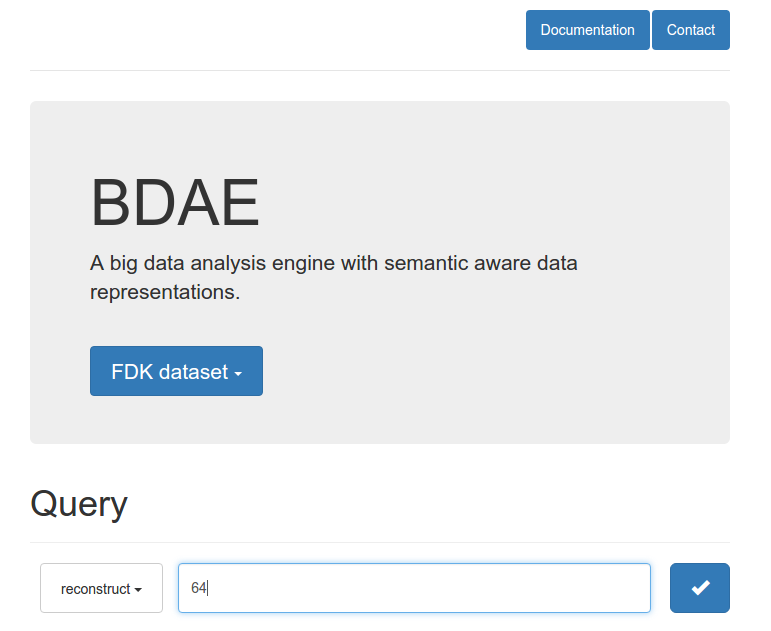
\includegraphics[scale=0.25]{../Report/img/website.png}}
\end{itemize}
\newslide

\myfullpage{Demo}{CT Reconstruction using SOFA + BDAE}
\newslide

% QUESTIONS PAGE
\myfullpage{Questions?}{}

\end{document}